\documentclass[12pt]{article}
\usepackage{indentfirst}
\usepackage{braket}
\usepackage{color}
\usepackage{graphicx}
\usepackage{graphics}
\usepackage{subfig}
\usepackage{amsmath}
\usepackage{amssymb}
\usepackage{geometry}
\usepackage{float}
\usepackage{ulem}
\usepackage{framed}
\usepackage{empheq}
\usepackage{mathtools}
\usepackage[linkcolor=blue,colorlinks=true,linktoc=all]{hyperref}
\makeatletter
\@addtoreset{equation}{section}
\makeatother
\renewcommand{\theequation}{\arabic{section}.\arabic{equation}}
%=========================================
\newcommand{\h}{\hbar}
\newcommand{\hr}{\hat{\rho}}
\newcommand{\dt}{\frac{d}{dt}}
\newcommand{\pt}{\frac{\partial}{\partial t}}
\newcommand{\K}{\ket}
\newcommand{\B}{\bra}
\newcommand{\BK}{\braket}
\newcommand{\tcb}{\textcolor{blue}}
\newcommand{\tb}{\textbf}
\newcommand{\ti}{\textit}
%==============================================

\graphicspath{{Diagrams/}}
\geometry{a4paper,scale=0.85}
\title{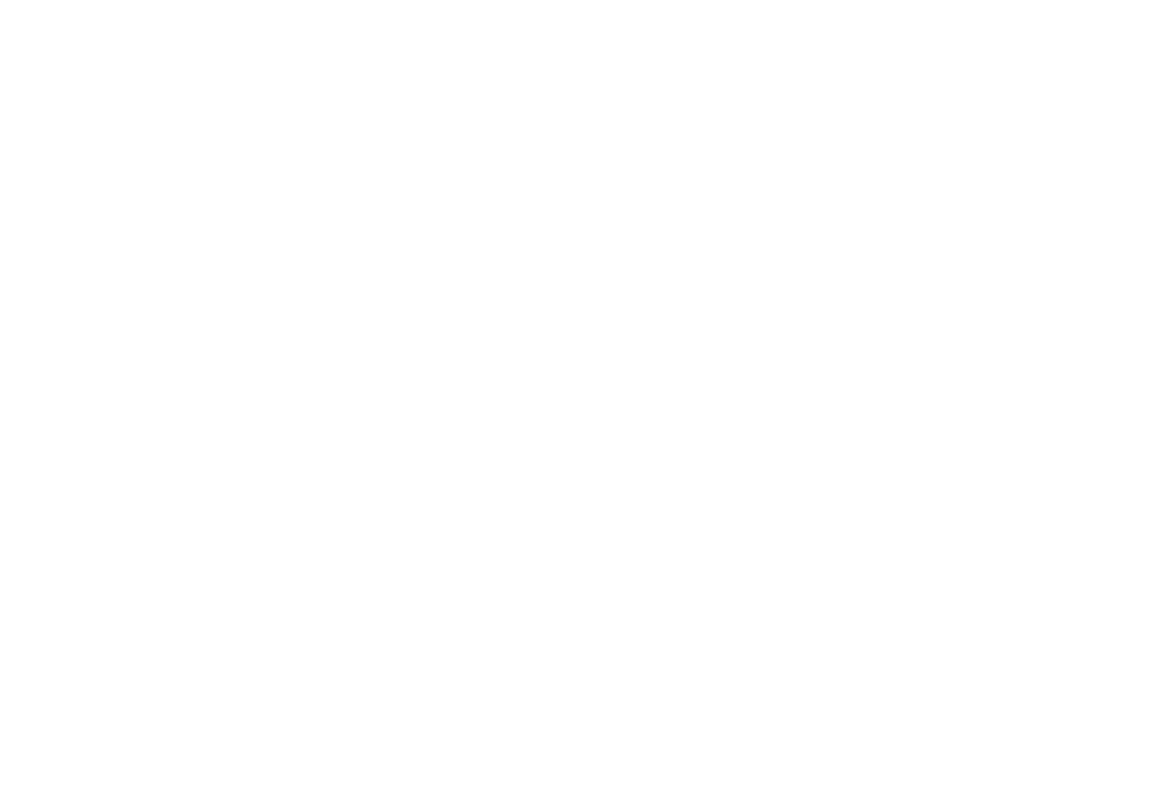
\includegraphics[scale=0.7]{0.pdf}\\ \Huge{\textbf{Spintronics Note\\}}}
\author{Guo Liangliang, \href{aoubleliang@gmail.com}{aoubleliang@gmail.com}\\ \\ \href{http://www2.phy.pku.edu.cn/~LabSpin/home.html}{WeiHan Group} of ICQM--Peking University}
\date{}
\begin{document}
\maketitle
\newpage
\tableofcontents
\newpage

\section{The Quantum Mechanics of Spin}
\label{sec: quantum mechanics of spin}
\subsection{Pauli Matrices}
\label{sec: pauli matrices}

We have the following relations 

\begin{subequations}
	\begin{empheq}[box=\fbox]{align}
		\begin{split}
			& [S_i,S_j ]=\varepsilon_{ijk} i \h S_k\\
			& S^2\K{s,m}=\h^2 s(s+1)\K{s,m}\\
			& S_z \K{s,m}=\h m \K{s,m}\\
			& S_{\pm}\K{s,m}=(S_x \pm i S_y)\K{s,m} =\h \sqrt{s(s+1)-m(m\pm1)} \K{s,m\pm 1}
		\end{split}
	\end{empheq}
\end{subequations}


We have two states for spin 1/2
\begin{align*}
	\alpha=\begin{pmatrix}
		1\\0
	\end{pmatrix}; \beta=\begin{pmatrix}
		0\\1
	\end{pmatrix}
\end{align*}

And we can know 
\begin{align*}
	S^2 \alpha=\frac{3}{4}\h^2 \alpha; S^2 \beta=\frac{3}{4} \h^2 \beta 
\end{align*}

Let $S^2=\begin{pmatrix}a &b\\c&d\end{pmatrix}$, then we can get 
\begin{align*}
	S^2=\frac{3}{4}\h^2	\begin{pmatrix}
		1&0\\0&1
	\end{pmatrix}
\end{align*}

Similarly, we can get 
\begin{align*}
	S_z=\frac{\h}{2}\begin{pmatrix}
		1&0\\0&-1
	\end{pmatrix}; S_+=\h \begin{pmatrix}
		0&1\\1&0
	\end{pmatrix}; S_-=\h \begin{pmatrix}
		0&0\\1&0
	\end{pmatrix}
\end{align*}

Or 
\begin{align*}
	S_z=\frac{\h}{2}\begin{pmatrix}
		1&0\\0&-1
	\end{pmatrix}; S_x=\frac{\hbar}{2}\begin{pmatrix}
		0&1\\1&0
	\end{pmatrix}; S_y=\frac{\hbar}{2}\begin{pmatrix}
		0&-i\\i&0
	\end{pmatrix};
\end{align*}

And we let $S=\frac{\hbar}{2}\sigma$, where $\sigma$ is what we call Pauli Matrix

\begin{align*}
\boxed{
	\sigma_z=\begin{pmatrix}
		1&0\\0&-1
	\end{pmatrix}; \sigma_x=\begin{pmatrix}
		0&1\\1&0
	\end{pmatrix}; \sigma_y=\begin{pmatrix}
		0&-i\\i&0
	\end{pmatrix};}
\end{align*}

Or to make it easer to remember, we get a generally form 
\begin{align*}
	\sigma_a=\begin{pmatrix}
		\delta_{a3}&\delta_{a1}-i\delta_{a2}\\
		\delta_{a1}+i\delta{a2}&-\delta_{a3}
	\end{pmatrix}
\end{align*}

where $\delta_{ai}$ is \tcb{Kronecker delta}. \\

After we get the Pauli matrices, we can correspondingly get their eigenstates which are:

\begin{gather*}
	\psi_{z+}=\begin{pmatrix}
		1\\0
	\end{pmatrix}; \psi_{z-}=\begin{pmatrix}
		0\\1
	\end{pmatrix}\\
	\psi_{x+}=\frac{1}{\sqrt{2}}\begin{pmatrix}
		1\\1
	\end{pmatrix}; \psi_{x-}=\frac{1}{\sqrt{2}}\begin{pmatrix}
		1\\-1
	\end{pmatrix}\\
	\psi_{y+}=\frac{1}{\sqrt{2}}\begin{pmatrix}
		1\\i
	\end{pmatrix};\psi_{y-}=\frac{1}{\sqrt{2}}\begin{pmatrix}
		1\\-i
	\end{pmatrix}
\end{gather*}


\subsection{The Pauli Equation and Spinors}
\label{sec: pauli equation}

We can set the electron' wavefunction as 
\begin{align}
	[\psi(\pmb{x})]=\begin{bmatrix}
		\phi_1(\pmb{x})\\ \phi_2(\pmb{x})
	\end{bmatrix}	
\end{align}

Where $\pmb{x}=(x,y,z,t)$. Then we can recast the Schrodinger Equation 
\begin{align}
	\Big (\hat{H}-i\hbar \frac{\partial}{\partial t} [I]\Big)[\psi(\pmb{x})]=[0]
	\label{equ: pauli equation}
\end{align}

This is a set of two simultaneous differential equations for the two components of the spinor wavefunction--$\phi_1$ and $\phi_2$. And this is referred to as the \tcb{\ti{Pauli Equation}}.\\ 

Right now, we can calculate the expected value of the spin components with special expressions. 
\begin{gather}
	\BK{S_n}=\frac{\hbar}{2}[\psi(\pmb{r},t)]^\dagger \sigma_n [\psi(\pmb{r},t)]
\end{gather}


Specifically, 
\begin{gather}
	\BK{S_x}=\frac{\hbar}{2} \begin{bmatrix}
		\phi^\dagger_1(\pmb{x})& \phi^\dagger_2(\pmb{x})
	\end{bmatrix} \begin{bmatrix}
		0&1\\
		1&0
	\end{bmatrix} \begin{bmatrix}
		\phi_1(\pmb{x})\\ \phi_2(\pmb{x})\end{bmatrix}=\hbar Re(\phi_1^\dagger(\pmb{x})\phi_2(\pmb{x}))\\
		\BK{S_y}=\hbar Im(\phi^\dagger_1(\pmb{x}) \phi_2(\pmb{x}))\\
		\BK{S_z}=\hbar (|\phi_1(\pmb{x})|^2-|\phi_2(\pmb{x})|^2)
\end{gather}






















\end{document}
